%!TEX root = ./cikm2016.tex
\section{Thompson Sampling on synthetic data}
In this section, we verify the sequential Thompson sampling through a compositional and non-compositional synthetic data sets.
\label{sec:thompson_synthetic}
\begin{figure}[t]
	\centering
	\subfigure[\scriptsize Logistic: N=10, K=10, D=5\label{fig:syn1}]{
	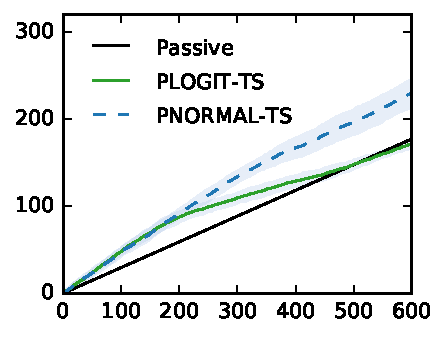
\includegraphics[width=0.43\linewidth]{images/toy_logit_vs_normal_10_10_5.pdf}
	}
	\subfigure[\scriptsize Logistic: N=20, K=10, D=5\label{fig:syn2}]{
	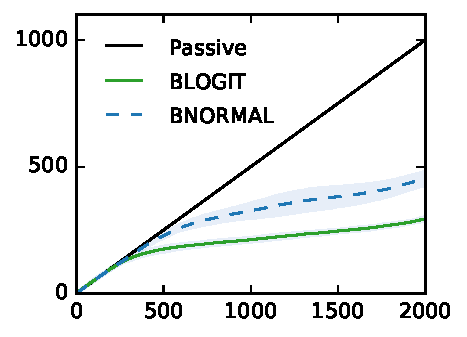
\includegraphics[width=0.45\linewidth]{images/toy_logit_vs_normal_20_10_5.pdf}
	}
	\subfigure[\scriptsize Gaussian: N=10, K=10, D=5\label{fig:syn3}]{
	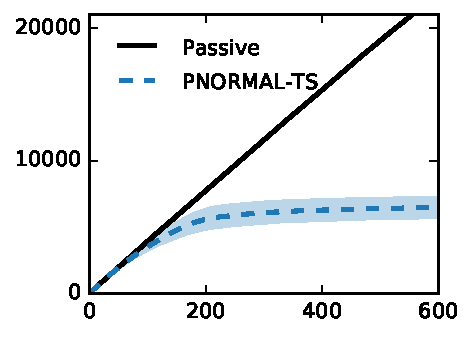
\includegraphics[width=0.45\linewidth]{images/toy_10_10_5.pdf}
	}
	\subfigure[\scriptsize Gaussian: N=20, K=10, D=5\label{fig:syn4}]{
	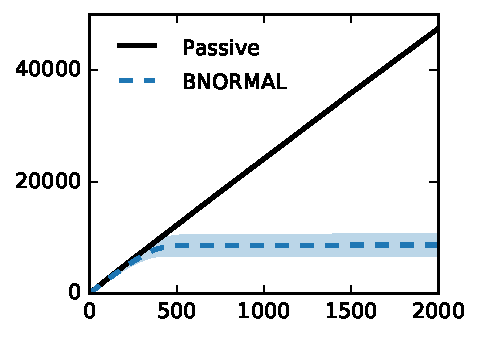
\includegraphics[width=0.45\linewidth]{images/toy_20_10_5.pdf}
	}
	\caption{\label{fig:synthetic} Cumulative regret of particle Thompson sampling with Gaussian and logistic output (PNORMAL-TS, PLOGIT-TS) against Passive learning
	on synthetic datasets with logistic	(top row, a, b) and Gaussian (bottom row, c, d) output variables.
	The averaged cumulative regrets over 10 runs are plotted with one standard error.
	As the model obtained more and more labeled samples from Thompson sampling,
	the cumulative regrets increase sub-linearly.}
\end{figure}

\begin{figure}[t]
	\centering
	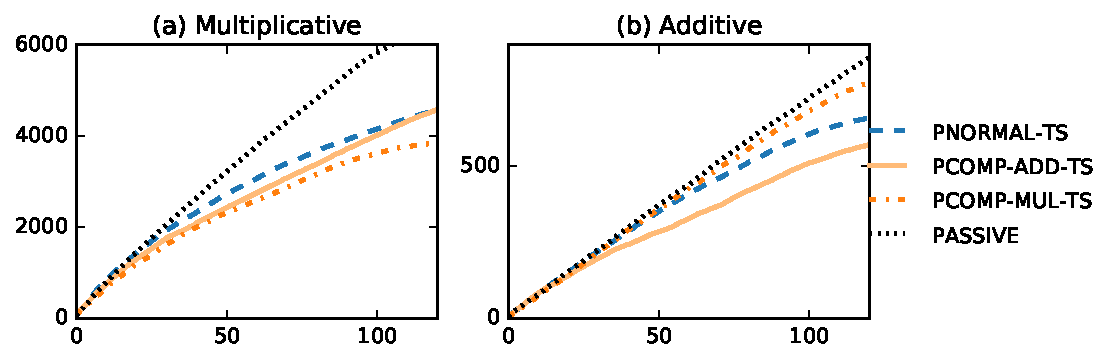
\includegraphics[width=\linewidth]{images/toy_comp_5_2_5.pdf}
	\caption{\label{fig:comp_synthetic} Cumulative regret of particle Thompson sampling of the compositional models on synthetic dataset with N=5, D=5. The synthetic dataset has three relations (K=3); the first two are independently generated, and the third relation is composed by the first two relations. The dataset used in (a) is generated by the multiplicative assumption, and the dataset used in (b) is generated by the additive assumption.}
\end{figure}

\subsection{Thompson sampling on non-compositional synthetic data}

We first synthesise two datasets
following the model assumptions in Section \ref{sec:brescal}.
\eat{We randomly generate triples based on randomly sampled entities and relations. Every }
\rev{First, }entities and relations are generated from zero-mean isotropic multivariate normal distribution, \eat{where we set }\rev{with }
variance parameters $\sigma_e=1$, $\sigma_r=1$ (Eqn. \ref{eqn:entity_gen} to
\ref{eqn:relation_gen}), respectively.
\rev{We generate two sets of \eat{the final}output triples,}
\eat{we generate two sets of datasets with }
\rev{with} the logistic output (Eqn. \ref{eqn:logit_triple_gen}) \eat{output variable }and the Gaussian \rev{with $\sigma_x$ set to 0.1}\eat{ variable} (Eqn. \ref{eqn:triple_gen}), respectively .
\eat{The variance of gaussian $\sigma_x$ set to 0.1.}

To measure performance\eat{ on synthetic dataset}, we compute cumulative regret
\eat{of proposed algorithm }at each time $n$ as $R(n) = \sum_{t=1}^{n} x_t - x^{*}_t$,
%\begin{align}
%R(n) = \sum_{t=1}^{n} x_t - x^{*}_t,
%\end{align}
where $x^*_t$ is the highest\rev{-valued} triple among triples that have not been chosen up to time $t$. Unlike the general
bandit setting where one can select a single item multiple times, in our formulation, we can select one triple
only once. So after selecting a triple at time $t$, the selected triple will be removed from a set of candidate
triples.

Figure \ref{fig:synthetic} shows the cumulative regret of the algorithm on the synthetic data with varying size of
entities and relations. We compare the cumulative regret of the particle Thompson sampling with the passive
learning method where the model choose a random triple at each time. All results are averaged over 10
individual runs with different initialisations.
Note that the dataset with binary logistic output variables can be used to train both logistic-output \textsc{Prescal} (\textsc{Plogit}) and Gaussian-output \textsc{Prescal} (\textsc{Pnormal}) whereas the dataset with the Gaussian output can only be trained by \textsc{Pnormal}.
Figure \ref{fig:syn1} and \ref{fig:syn2} show that with the logistic synthetic dataset both models are capable to learn the latent features of the generated triples, with logistic outperforming the Gaussian; Figure \ref{fig:syn3} and \ref{fig:syn4} show that the Thompson sampling for \textsc{Pnormal} (\textsc{Pnormal-ts}) \rev{outperform the passive learning in} the real valued dataset.
%For every experiment, the cumulative regret of the Thompson
%sampling method was bounded after a certain number of interactions whereas the cumulative regret of
%passive learning increases linearly.
\eat{Both results indicate the particle sampling is capable of inferring latent features
of entities and relations as the interaction increases.}

\subsection{Thompson sampling on compositional synthetic data}

We conduct a second experiment on synthetic dataset to understand how
the Thompson sampling works for the compositional data.
As in the first experiment, we first generate entities and relations from
zero-mean multivariate normal with variance parameter $\sigma_e = 1$ and
$\sigma_r=1$. We generate a set of triples with Gaussian output as in
Equation \ref{eqn:triple_gen}. We then synthesise two sets of expanded tensors
using the previously used entities and relations based on the multiplicative
and additive compositional assumptions, defined in Sec \ref{sec:comp},
respectively. So we synthesise fully observable expanded tensor $\mathcal{X}^L$
where $L=2$. We set both variance parameter $\sigma_x$ and $\sigma_c$ to 0.1.
Note that in a real world situation, the expanded tensor can only be constructed
through the observed triples, and the triples in the expanded tensor cannot be queried.

To run the particle Thompson sampling on the synthetic dataset, we let the
compositional models know which relation is composed by other relations.
The non-compositional \textsc{Pnormal} model assumes each relation is independent to one another.
Therefore, the compositional model uses much less number of parameters to model
the same size of tensor to compare with the non-compositional model.
\eat{%%LX: these info repeats?
Through
this experiments, we verify the particle Thompson sampling algorithm for the
compositional models.

For the experiment, we generate three relations ($K=3$) of five entities ($N=5$):
the first and second relations
are independent and the third relation is composed by the first and second
relations. The latent dimension is set to 5.
}
With this fully observable expanded tensors, we run the Thompson sampling of
the compositional models.
Figure \ref{fig:comp_synthetic} shows the cumulative regrets on synthetic
datasets. The multiplicative and additive compositionality are used to
generate the dataset for Figure \ref{fig:comp_synthetic}(a) and
\ref{fig:comp_synthetic}(b), respectively. The results correspond to our
assumption: the Thompson sampling for multiplicative compositional model (\textsc{Pcomp-add-ts}) shows lower
regrets on the multiplicative data in Figure \ref{fig:comp_synthetic}(a), and
the Thompson sampling for additive compositional model (\textsc{Pcomp-add-ts}) shows lower regrets on the
additive compositional data in Figure \ref{fig:comp_synthetic}(b),
and both have lower regrets than passive learning or \textsc{Pnormal-ts} without compositions.


\section{Posterior variance analysis}
\begin{figure}[t]
	\centering

	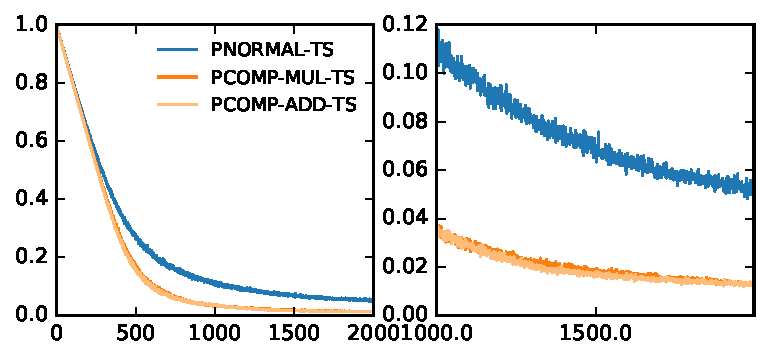
\includegraphics[width=0.9\linewidth]{images/posterior_variance_trace_kinship.pdf}

	\caption{\label{fig:pos_var} Trace plot of mean posterior variance of the non-compositional model and compositional models. Y-axis denotes the average posterior covariance, and X-axis denotes the number of queries. The second plot magnifies the first plot.}
\end{figure}

In section \ref{sec:exp2}, we find that the compositional model performs worse than the non-compositional models in the active incremental population. 
We emphasise the difference between two experiments;
the goal of incremental population is to maximise the number of triples
whereas the goal of knowledge completion in Section \ref{sec:exp1} is to maximise
the predictive performance. Nevertheless, the compositional models do not outperform
\textsc{Pnormal-ts} in the active learning.
This result can be partially understood in terms of the balance between
exploration-exploitation. Figure \ref{fig:pos_var} shows the average posterior variance of
the entity vectors. We compute the eigenvalues of posterior covariance matrix $\Lambda_i^{-1}$
and trace the average eigenvalues over the iterations.
As shown in the figure, the average variance of the compositional model shrinks much faster
than the \textsc{Pnormal-ts}. Because the exploration-exploitation of the Thompson sampling depends on the
posterior uncertainty, the fast shrinkage in the posterior variance may indicate the under
exploration of the model. This is predictable to a certain extent in the sense that one new triple with the compositional models induces multiple new
compositional triples, so the uncertainties of entities and
relations are measured less than those with non-compositional model. Most active
learning algorithms utilise model uncertainty, and hence a model with augmented
structures such as the relation compositions should be more careful about reflecting its uncertainty correctly.
